% TODO chapter6 is too large! split it into articles.
% \label goes always after \caption!!
\chapter{组织与管理}
\section{公司简介}
公司形式: 有限责任公司

\section{公司的核心价值观}
核心价值观是企业文化的重要组成部分,是企业的灵魂。它使企业有了克服困难的
勇气,开拓市场的魄力,不断创新的动力。公司的核心价值观总结为:
%
\begin{center}
        客户至上,敢于创新,\\追求卓越,勇攀高峰。
\end{center}
%
公司把核心价值观作为员工行动准则的一部分,写成标语贴在贴上;做成书签送给
员工;提在画上挂在墙上;喊在嘴里做在事里。只有这样,全公司上上下下才能团结一
心,奋勇当先,争创佳绩。

\section{公司目标}
为广大的亲子提供一流的餐饮体验是我们为之奋斗的目标。我们全公司上到管理
层,下到一线员工,无不秉持这一目标,努力为每一个前来就餐的家庭提供同样优质的
服务。我们虚心接受每一位顾客的监督,接受他们的意见和建议,以此不断改进管理制
度,不断推出新颖的菜肴,不断提升服务质量。我们也欢迎各位消费者朋友们通过微信,
QQ,热线电话和邮件反馈宝贵的建议,我们的联系方式是:

\begin{tabularx}{\textwidth}{@{\hspace{2em}}ll}
        微信公众号 & 爱厨艺亲子主题餐厅 \tabularnewline
        QQ &  19723110094 \tabularnewline
        热线电话 &  22213313 \tabularnewline
        邮箱 &  \url{ichuyi@126.com} \tabularnewline
\end{tabularx}

\section{公司组织结构}

\subsection{公司初期组织结构}
由于创业初期公司的规模较小,适宜采用直线型结构,这种结构能够做到快速决策,
机动灵活,降低管理成本。如图~\ref{fig:early-struct}所示。

% TODO Draw this structure graph in latex
\begin{figure}[htbp]
        \centering
        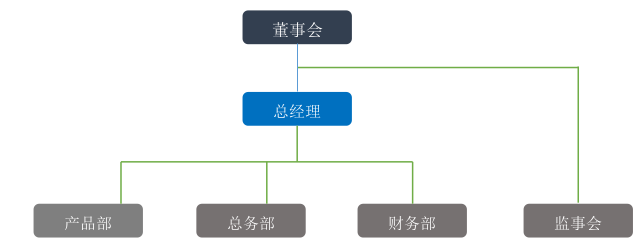
\includegraphics[width=0.8\textwidth]{../images/company/早期结构}
        \caption{公司初期组织结构图}
        \label{fig:early-struct}
\end{figure}
\paragraph{董事会}
属于决策层,由公司的主要股东组成。负责制定公司整体发展战略,任命
总经理。它由 8 名成员组成,其中投资者和公司的初始风险团队按照股份分配。公司管
理层董事人数应占董事会半数以上。董事任期为三年。一旦任期届满,他们可以连任。

\paragraph{监事会}
没有监督的权力是危险的。因此,还有一个与监事会设立相对应的监事会,
它监督董事会主席,以保证股东的权益。监事会成员由股东和公司员工代表组成。有 5
名成员,其成员中有一名召集人。监事会中股东代表监事与职工代表监事比例为 3:2。
监事会的股东代表监事由股东大会选举产生,职工代表监事由公司职工民主选举产生。
监事任期三年。任期届满时,可以连选连任。

\paragraph{总经理}
主要负责制定公司的重大战略决策,负责整个公司的正常运作,有责任创
造良好的企业文化,承担团队建设的责任,协调各部门的工作,履行绩效评估负责组织
部门负责人,组织公司月度,季度,年度计划和指标的编制工作,监督各部门的运作和
发展情况,监测公司人力资源状况,财务收支情况和公司整体资产状况。

\paragraph{秘书处}
协助总经理处理公司日常事务作为工作中心,协调各部门之间的关系,促
进公司各项工作的顺利开展,并负责人员出勤和其他方面的工作。同时,它在公司中起
着上传和发布的作用。

\paragraph{营销部}
负责公司市场开发和营销计划的制定,组织实施市场调
研和相关数据分析,按照公司的经营目标和长期计划制定年度经营计划,并负责市场调
研推广产品和服务,促进业务目标的有效实现。协助客户服务部门维护与客户的关系,
及时提供市场动态,协助规划部门开展相关活动。

\paragraph{产品部}
负责新技术的创新和研发,以及现有技术的更新。根据市场需要生产出合
格的产品,并重视新产品的创新开发。负责产品研发,拓展产品线的广度和深度。负责
新技术的开发和推广。负责某些产品的售后技术支持。

\paragraph{财务部}
负责公司财务,会计和税务事宜。基于健全的财务管理原则,本行将发挥
财务管理职能;制定财务计划和预算制度;有效规划和使用公司资金,维护账户的登记和
安排,编制财务报告,提供管理部门决策所需的信息。

\paragraph{总务部长}
由于组织的减少,总务部完成了其他辅助功能。包括:信息管理,物流
服务,外包服务包括法律咨询等。起草和总结公司各种管理制度,负责组织工作分析,
并提供相应的解决方案。负责组织招聘和确保招聘优秀员工。制定培训体系,开展员工
培训。负责部门工作人员的管理和考核,参与公司年终考核;保留人事档案;协调与公司
其他部门的关系,做好有关人员信息的交流工作。




\subsection{公司中后期结构}
\begin{figure}[htbp]
        \centering
        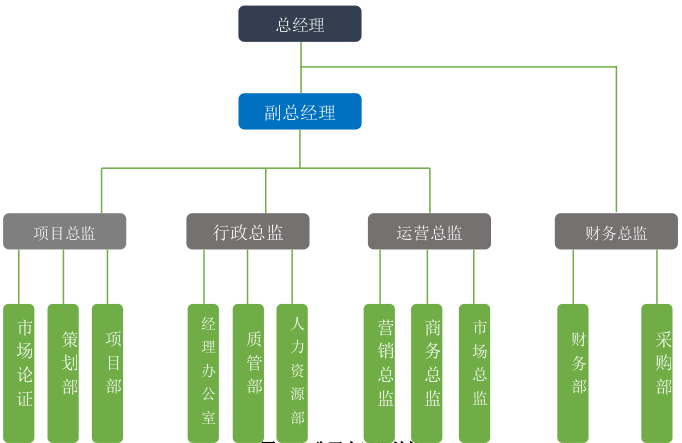
\includegraphics[width=0.8\textwidth]{../images/company/后期结构}
        \caption{公司中后期结构}
        \label{fig:late-struct}
\end{figure}




在创业发展阶段(公司成立后 3 年到 5 年)原来的那种集中式组织结构将会限制
企业进一步发展。这时我们将会进行组织变革,将企业组织管理战略与企业总体战略相
匹配。企业由直线制结构由职能式结构转变为三级项目办公室,如图~\ref{fig:late-struct}
所示。 这种管理结构有利于加强项目间的协调和标准化。 这是公司在开发阶段不断开设
分店的良好模式。 公司进入成熟阶段(第五年以后)时,子公司的数量和规模不断扩
大。 控制和评估每个子公司将更加困难。 此时,将建立业务部门以适应公司的规模。

\section{管理形式}
\subsection{管理团队和基本思想}
本公司的创业团队由北京航空航天大学烹饪协会和计算机系的六名本科同学构成,
由专业的老师为我们做运营指导。我们将构建一支在有爱心、有耐心、踏实上进的队伍,
欢迎一切有志于亲子主题餐饮的人才加入本公司。

\paragraph{管理思想}
作为一家新型餐饮类企业,我们重视员工个人的发展, 努力为员工开拓更大的发展
空间;我们认为员工的发展和公司的发展是统一并且相辅相成的。我们强调各职能部门
相互协调合作, 在管理层的协调和调度下,为公司的经营打下坚实的基础。

\paragraph{管理决策}
公司初期的管理团队主要由创业团队人员组成。团队成员都是在读的北京航空航天
大学本科生, 来自计算机、法律、经济管理等专业,具有烹饪爱好。我们乐观上进,积
极进取,将为公司制定切实可行的决策, 并且坚定不移的执行。在获得风险投资后, 投
资者自然也以股东的形式成为公司的管理顾问;我们还将聘用具有丰富管理经验的人才
担任重要职务。

\paragraph{管理理念}
\begin{center}
        关心员工成长, 强化执行能力,\\
        追求高效和谐, 平衡激励约束。
\end{center}

\paragraph{关心员工成长}
重视员工的兴趣和专长,以良好的工作条件、完善的员工培训计划、职业生涯通道
设计促进员工个人职业发展;重视企业文化管理,以健康简单的人际关系、严肃活泼的工
作气氛、畅快透明的沟通方式,促进员工满意度的不断提高,使员工保持与企业同步成长
的快乐;激发员工潜能,追求个人与公司共同成长。作为个人要有先付出的意识,甘于为
团队奉献智慧和勤奋,以优秀的团队成就个人的优秀。

\paragraph{强化执行能力}
再好的研究策划,没有好的执行就会成为空谈。强力执行是创业在管理上的核心原
则之一;良好的执行力,要依靠优秀的机制、规范的制度、精诚的合作、有效的激励、感
人的榜样,但最重要的,要依靠每位创业人对公司的热爱和对工作的负责精神。

\paragraph{追求高效和谐}
根据公司发展阶段和业务变化,动态优化企业的管理,形成和谐有序的内部环境;在
高效与和谐的环境下,坚持结果导向的管理原则,有效支持公司经营目标的实现。

\paragraph{平衡激励约束}
根据工作贡献和成果价值, 形成差异化的激励机制,有效激发员工的主观能动性和
创造性;强调激励与约束相结合、保持平衡有度,为实现内部管理提供有力保障。

\subsection{岗位说明书}
职位管理是一个复杂的系统。最基本的手段是定义和解释责任范围。每个职位都有
自己的主要职责,然后进行一些协调的工作。为了让员工明确自己的任务和责任,公司
将为每个职位准备工作描述。首先,职位描述清楚地列出了员工责任的范围。通过他的
工作描述,他可以理解他的工作职责。其次,职位描述包括员工的需求,员工可以在这
些领域控制自己的发展,以及哪些能力还需要进一步改进。第三,职位描述使上下级之
间的工作关系明确。第四,职位描述也有利于评定员工的优秀程度。负责招聘新员工和
评估老员工的表现,他们都可以参考职位描述的要求。它可以确定职位的工作资格,为
设计培训计划提供依据,并为绩效评估提供基础依据。公司将实施严格的问责制度。每
个员工都必须知道他的工作要求和责任范围,谁负责的任务,就向谁问责。

\subsection{公司的规章制度}
建立一套行之有效的规章制度是公司生存发展的必要条件,是形成企业文化的基
础,是塑造公司核心价值观的保证。因此,公司将考虑各部门的要求和建议,制定出具
有可操作性,可执行性和人性化的法规。在制定制度的过程中,我们将与全体员工充分
沟通,使制度得到保证。公平合理也可以得到员工的支持和理解。公司将在其所有法规
中体现激励和责任的原则。严谨谨慎的系统设计反映了公司的人文关怀和创新激励,同
时恶意破坏公司的核心价值和其他违规行为。按照规则行事。

一旦公司的系统建立起来,它就不会轻易改变。如果有任何改变,将遵守相关程序,
并及时告知员工培训新员工的核心问题之一是熟悉公司的规章制度和行为标准。人事部
门不仅将所有公司的规章制度和行为准则逐一分析给新员工,所有员工也必须严格执行
工作。他们必须将规章制度变成一种意识,并将规章制度付诸行动,成为习惯。



\section{企业文化}
\subsection{团队标志}
% All I need is to place this company-logo in front of the introduction.
% The use of float (figure) went mad with it. One solution is to use the
% float package, its [H] specifier, but that goes too far. All I want is
% the caption, so the capt-of package is handy for adding caption to non-float.
% This logo looks nice without being a float.

\begin{center}
        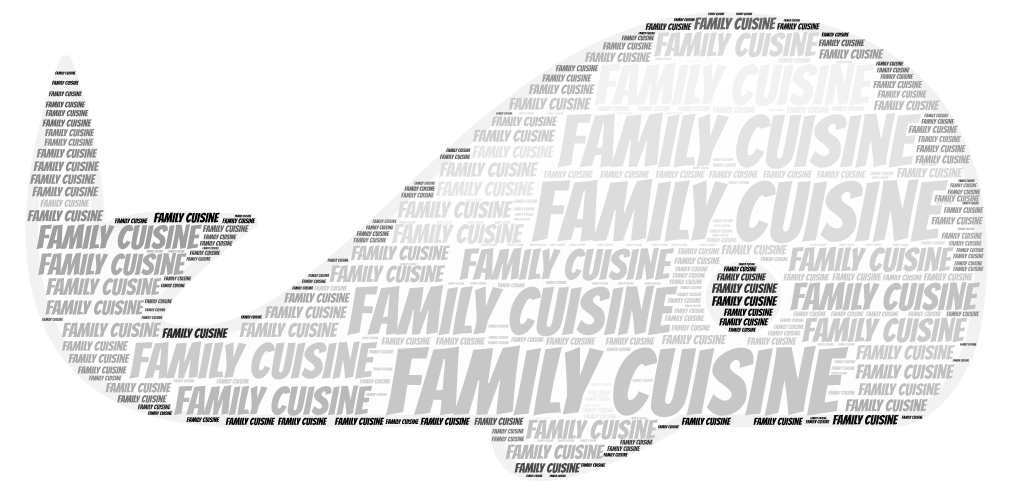
\includegraphics[width=0.3\textwidth]{../images/company-logo}
        \captionof{figure}{北京爱厨艺餐饮有限公司标志}
        \label{fig:company-logo}
\end{center}

标志解读: Family Cuisine 是公司的英文名,意思是“一家人的菜肴”。公司的主
要经营项目是“北京爱厨艺亲子主题餐厅”,这个图标突出了公司以亲子为中心的理
念。鲸鱼的外形象征着活力、健康和和睦;参差不齐的字形象征着孩子活泼爱玩的天性。
图标寄寓着公司对顾客的家庭幸福和睦的祝福。

\subsection{企业文化理念}
\paragraph{质量}
建立企业声誉,最重要的是产品的整体质量。要提高食品质量,活动质量,环境质
量和服务质量,提高产品的整体质量,提高餐饮附加值,实现消费者满意。

\paragraph{廉正}
这是中华民族的传统美德,也是建立企业品牌的基石。要坚持“诚实守信,开放负
责”的职业道德,重视公司在行业和市场的信誉,注重提高企业声誉,切实履行应尽的
责任。管理,运营和食品采购方面。遵守社会道德标准,在社会承诺和经营行为方面充
分考虑客户的需求和利益,提高公司在行业和市场上的品牌声誉。

\paragraph{卓越}
体现公司精神,追求卓越品质,具有远大抱负和高瞻远瞩的认知能力,体现公司的
理想和追求。我们的职业生涯是一场从平庸到卓越,再到非凡的斗争。我们必须始终保
持“追求卓越”和“敢于超越”的理念和勇气。通过保持先进感,我们将提高产品质量,
超越自我,超越竞争对手,并最终将平庸转化为卓越和非凡。

\section{人力激励与约束机制}
\subsection{激励机制}
\paragraph{保持良好的薪酬体系}
餐饮公司的员工教育水平相对较低,一般更关心物质激励。 员工用自己的报酬来衡量
自己的价值,相对工资水平也影响员工的公平感。 尽管薪酬和福利不足以激励员工,
但他们是必要的工具。

\subparagraph{体现公平}
当员工对薪酬制度感到不公平时,可能会采取一些负面的反应,如减少责任和辞职。
公平的补偿制度不仅包括内部公平,还包括外部公平。

\subparagraph{激励}
餐饮公司是相对低收入的公司。因此,他们可以采用高度稳定的薪酬模式,提高基
本薪酬和保险福利的比例,降低绩效薪酬比例,使员工感到安全。绩效工资必须保持可
用,评估指标必须具备客户满意度,劳动时间和其他关键指标。公司在指定激励制度时
必须有明确和一致的原则,并且应该有统一和可执行的准则作为基础。激励头寸之间的
工资差距必须有一定的基础和全面合理。为降低员工离职率和留住核心人才,公司可以
采取具有长期激励效应的薪酬体系,如员工持股和股票期权(ESO)。

\paragraph{补充使用心理奖励}
奖励是员工需求的满足。员工的需求多种多样,因此激励措施各不相同。应允许物
质激励和精神激励相辅相成。

\subparagraph{工作目标奖励}
目标是衡量员工的工作表现。在食品和饮料行业,管理人员应该
为员工制定服务标准或提出要求作为工作目标。

\subparagraph{工作流程奖励}
管理者应该经常向员工灌输正确的专业观点,并经常赞扬和鼓励
员工。另外,员工也应该被允许去做他们最喜欢的工作。他们可以通过轮换或张贴来丰
富自己的角色,这样员工就可以找到自己的兴趣爱好,并尽力让他们在自己最喜欢的职
位上做自己喜欢的工作。

\paragraph{工作完成激励}
对于一些优秀的员工来说,例如某种创新菜的销售量很高,或者
服务得到客户的赞扬,餐厅经理或厨师可以给员工一些小礼物,例如配方,新配料。工
作服,一个美丽的新厨房,等等。但是,它必须是实用的而不是浮华。

\subparagraph{荣誉奖励}
对于员工来说,一方面他们获得较高的评价和尊重,就会产生一种成就感和心理满
足感和自我实现感。另一方面,荣誉也意味着未来一个人获得更好的收入的可能性,因
为一个人过去的工作的良好声誉可能会使他在当前的工作企业中获得更高的印象。

\subparagraph{建立科学的人才选拔机制}
适当运用内部促进,坚持公开,公平,公正的原则,
为内外部人才吸引和选拔实际人才提供平等机会,逐步摆脱“家长制”管理模式。

\subparagraph{完善培训机制}
员工培训应侧重于公司服务的特点。它不仅要强调企业服务知识的培训,还要强调
人际交往技能的培养,包括沟通技巧,冲突解决能力和跨文化敏感意识。考虑到餐饮业
的长远发展,餐饮业的安全性和员工忠诚度的培养,公司内部培训是一种符合成本核算
原则的明智举措。

\subsection{约束机制}
就治理结构而言,仅有激励措施是不可行的,有时激励措施是好的,但也存在人力
资本运作不好的问题。 因此,在建立激励机制的同时,还必须建立约束机制。 人力资
本的约束机制大致可以分为内部约束和外部约束两个方面。

\subparagraph{内部约束}
内部约束是公司和人力资本之间的约束,以及各方之间的约束。
从国际上看,这种内部制约主要有四个方面的约束措施。该公司的章程是有约束力的。
当人力资本进入一家公司并且公司受到制约时,第一个约束就是公司的宪法规定,这意
味着公司的每个人都必须服务并提交给公司章程。合同限制。企业中的任何人力资本都
必须签署非常详细的合同。这种合同必须表现出对公司商业秘密的保护,对技术专利的
保护以及对竞争力的保护。偏好约束。所谓的偏好约束,就是我想约束你,首先要考虑
你的偏好是什么。如果你想实现自己的经营理念,而不是更多的钱,那就用它来强化你,
来约束你。制度约束。所谓制度约束是指高度重视改善企业的最高决策机构。人力资本
与企业之间的摩擦和矛盾必须发生,成人与机构之间的矛盾应该得到发展。企业与人力
资本之间的矛盾之所以不能转化为人与人之间的矛盾,是因为人与人之间的摩擦难以使
人力资本受到正常的约束。更重要的是,这种限制往往会增加。在个人的好恶之中,往
往需要将人与成人之间的摩擦转化为组织间的摩擦,这必须高度重视公司决策机构的完
善。

\subparagraph{外部制约因素}
所谓的外部制约因素实际上是社会制约因素,即人力资本形成
中的社会制约因素。该约束通常具有以下几个方面:法律约束。公司全体员工必须遵守
有关法律法规,诚实守信,依法行事。道德约束。每个阶层都应该有自己的职业道德,
所以人力资本也应该受到道德上的制约。市场约束。人力资本作为一种资本流经人力资
本市场。这种市场在遏制人力资本方面应该起到非常重要的作用。社会群体约束。所谓
的社会群体约束意味着作为人力资本,它应该有自己的非政府组织,因为民间社会组织
实际上是市场约束和道德约束之间非常重要的约束。媒体限制。媒体限制必须遵守促进
某些新闻的标准。应该有利于企业的发展。它必须考虑企业的负担能力和收益,不应该
炒作。

